Tato kapitola popisuje celkovou koncepci vlastního senzoru pro měření
rychlosti hnacího vozidla -- tzv. měřicího vozu. Dále popisuje
a zdůvodňuje rozhodnutí, která autor při konstrukci senzoru zvolil.

V~kontextu následujícího textu si autor dovoluje připomenout Požadavky
na řešení (kapitola \ref{chap:pozadavky}).

\section{Umístění senzoru}
\label{sec:wsm-senzor-umisteni}

Prozkoumejme nejprve kam je a~kam není možno senzor umístit. Určitě platí, že
senzor není možné umístit do lokomotivy. Lokomotiva je totiž komerční produkt,
který umožňuje úpravy její elektroniky nejvýše na úrovní výměny digitálního
dekodéru DCC. Lokomotiva obvykle bývá vybavena deskou plošných spojů, která
propojuje jednotlivé součásti lokomotivy (motor, koleje, dekodér, osvětlení,
...), tato deska je specifická pro konkrétní model a~dodává ji výrobce hnacího
vozidla. Zasahovat do elektroniky lokomotivy je tedy vysoce nepraktické a
mnohdy i~nemožné.

Druhou možností je doplnit senzor do lokomotivy bez úpravy její elektroniky.
To s~sebou ale nese pořád tu nevýhodu, že je třeba mechanicky zasahovat do
(poměrně drahé) lokomotivy.

Třetí možností je umístit senzor mimo hnací vozidlo. Senzor může být
umístěn na kolejiště staticky (podobně jako v~\ref{sec:det-static}) nebo může
být součástí vagónu připojeného za lokomotivou. Statické senzory jsou nevyhovující
zejména proto, že neumožňují provádění dokalibrace za skutečného provozu.

Jako nejvhodnější řešení se tedy jeví vyrobit vůz, který se připojí ke kalibrované
lokomotivě jako běžný vagón. Součástí tohoto vozu bude senzor pro měření
rychlosti. Vůz pak bude možné připojit bez narušení provozu i~za vlak na
\uv{produkčním} kolejišti.

S~uvážením výše uvedených argumentů se autor rozhodl vydat cestou
\textit{měřicího vozu}.

\section{Senzor}
\label{sec:wsm-senzor}

Důležitou součástí měřicího vozu je rychlostní senzor. Zvolená technologie
senzoru ovlivňuje formát a~přesnost měření, dále pak mechanicko-elektrické
vlastnosti měřicího vozu, jeho cenu, snadnost výroby, opakovatelnost výroby
(dostupnost součástek s~výhledem na několik let) a~v~neposlední řadě
poruchovost a~servisovatelnost měřicího vozu.

Autor uvážil několik dostupných technologií senzorů.

\subsection{Magnetický senzor}
\label{subsec:wsm-senzor-mag}

První uváženou technologií jsou tzv. \textit{magnetické poziční senzory}.
Tyto senzory fungují na bázi hallových sond. Umí měřit úhel natočení objektu
vzhledem k~senzoru. Jejich primárním účelem je měřit natočení nejrůznějších
ramen, či prvků ovládaných např. servomotory, opakovaným měřením natočení lze
ale dosáhnout také velice přesného měření rychlosti. Princip těchto senzorů
dobře ilustruje obrázek \ref{fig:magnetic-sensor}.

\begin{figure}[h]
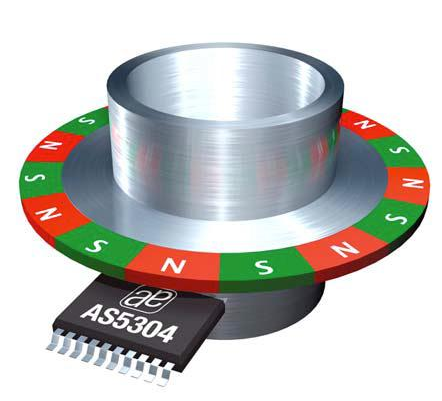
\includegraphics[width=0.5\textwidth]{data/magnetic_sensor.png}
\caption{Ukázka principu činnosti magnetického senzoru, převzato
z~\cite{as5306}.}
\label{fig:magnetic-sensor}
\end{figure}

Výhodou tohoto způsobu měření je velice vysoká přesnost (řádově 10 bitů na
jednu otáčku). Bohužel, při pohledu na obrázek \ref{fig:magnetic-sensor} je
velice těžko představitelné jak umístit senzor na nápravu vagónu. Senzor by
musel být umístěn z~boku vozu, což by výrazně snižovalo jeho stabilitu.

Existují ale i~senzory, které se montují přímo na osu rotujícího předmětu viz
například senzor \textit{AS5306} \cite{as5306}. Takový senzor by pro účel této
práce byl nejvhodnější. Nepříznivým faktem ale je, že tyto senzory vyžadují
magnetický disk, z~nichž nejmenší dosahují průměrů řádově $15\ mm$
\cite{magnets}. Tento průměr je pro modelovou železnici bohužel příliš velký.

\subsection{Magnetický senzor \uv{cykloměřič}}
\label{subsec:wsm-senzor-cyclo}

Technologie tzv. \uv{cykloměřiče} byla historicky první metodou jak měřit
rychlost modelové lokomotivy. Tento senzor autor dokonce viděl v~praxi, je
založený na stejném principu jako počítač rychlosti na cyklistickém kole.  Na
osu nápravy je upevněn magnet, ve voze je pak hallova sonda. Magnet vyvolá při
průchodu kolem hallovy sondy zákmit v~magnetickém poli, který tato sonda
detekuje. Na jednu otáčku nápravy tak připadá jeden zákmit, cyklopočítač pak
počítá počty zákmitů.

Toto řešení je poměrně jednoduché na instalaci, množství mechanických prvků je
malé, na druhou stranu ale poskytuje poměrně malou přesnost -- zejména při
nižších rychlostech. Technologie \uv{cykloměřiče} se tedy pro potřeby této
práce také nejeví jako vhodná.

\subsection{Optický senzor}
\label{subsec:wsm-senzor-opto}

Třetí zvažovanou technologií je optický senzor. Tento senzor je proslulý svým
užitím v~optických myších, pracuje na principu snímání obrazu podložky CCD
čipem a~porovnávání dvou obrazů pořízených v~krátkém časovém intervalu za
sebou. Ze dvou obrazů je pak určen rozdíl polohy myši. \footnote{Zajímavostí
je, že celá logika porovnávání dvou obrazů je v~takovýchto senzorech
implementována hardwarově.}

Toto řešení vypadá velice slibně, jeho obrovskou výhodou je absence jakýchkoliv
mechanických částí. Stačí namířit senzor na pražce a~jednoduše měřit jak se vůz
pohybuje. Pražce jsou navíc vůči štěrku mezi pražci velice dobře kontrastní,
porovnávání obrazů by tak mohlo být přesné (srovnejte s~pohybem optické
myši po takřka uniformním povrchu stolu nebo podložky pod myš).

Pro kalibrační vůz byl vybrán senzor \textit{ADNS-3050} \cite{adns-3050}.
Tento senzor byl mezi mnohými podobnými zvolen proto, že (1) má výstup sériovou
linkou a~(2) zvládá měřit vysoké rychlosti (vagón se typicky pohybuje o~něco
rychleji než myš).

Autor zakoupil senzory, osadil je na desku plošných spojů a~začal testovat
přesnost měření pomocí jednoduchého zapojení s~vývojovým kitem Arduino. Nemalou
výzvou bylo sehnat čočku, která autorovi umožní zaměřit pražce a~zároveň
ponechat senzor na ploše vagónu. Díky spolupráci s~Ústavem přístrojové techniky
AV ČR se však povedlo dostatečně malou čočku obstarat.

První měření ukázala, že pro dobrou funkci senzoru je třeba poměrně kontrastní
snímaná plocha a~poměrně intenzivní červené světlo (na to je CCD čip v~senzoru
nejcitlivější \footnote{Proto si optická myš přisvětluje červeným světlem.})
Navíc se ukázalo, že hloubka ostrosti senzoru je nejvýše $1\ mm$, což reálně
znemožňovalo měřit rychlost na kolejích, které nejsou zasypány štěrkem, ale
pouze připevněny k~podložce. Složitý optický senzor tak degradoval na zařízení,
jehož funkci by v~podstatě šlo obstarat pomocí jedné LED diody a~jednoho
fototranzistoru \footnote{Stačí jednoduše měřit intenzitu odraženého světla a
zkoumat, jestli je senzor zrovna na pražci nebo mezi pražci.}.

Po několika měsících pokusů o~zprovoznění měření optickým senzorem autor naznal,
že s~tímto typem senzoru nebude schopen garantovat přesné a~spolehlivé měření.
Padlo tedy rozhodnutí tuto technologii opustit. Autor by rád zdůraznil, že
jednou z~hlavních motivací pro opuštění této technologie byla přílišná
komplexnost senzoru a~neschopnost ovlivňovat a~debugovat procesy uvnitř něj.

\subsection{Optozávora}
\label{subsec:wsm-senzor-optozavora}

\begin{figure}[h]

\includegraphics[width=0.3\textwidth]{data/clonka.pdf}
\caption{Příklad paprskového kola.}
\label{fig:wheel}
\end{figure}

Čtvrtá uvažovaná technologie senzorů je inspirována návrhem od kolegy modeláře
Petra Trávníka. Jejím základem je paprskové kolo \ref{fig:wheel}
upevněné na nápravě měřicího vozu. Paprskové kolo se otáčí spolu s~nápravou,
k~vozu je pak připevněna optozávora, která snímá průchod jednotlivých paprsků.
Klíčovým faktorem pro použitelnost této technologie jsou zejména technické
možnosti výroby dostatečného množství paprsků při zajištění rovnoměrnosti
rozestupu paprsků a~malé velikosti kola. Průměr kola by totiž neměl přesáhnout
$6\ mm$ (pro měřítko TT, 1:120).

Tato technologie sice obsahuje mechanické prvky, ale pořád je jich poměrně
málo, při dostatečném počtu paprsků dosahuje dobré přesnosti, je jednoduchá, a
tudíž jsou data z~ní snadno zpracovatelná. Optozávora je také levná a~relativně
snadno dostupná.

Ze všech zvažovaných technologií autor nakonec zvolil právě technologii
paprskového kola a~optozávory.

Nejvhodnější technologií pro výrobu takového kola je zřejmě leptání, protože
autor však nemá k~této technologii přístup, rozhodl se místo jednotlivých
paprsků kolo vyrobit dírkované. Jako vhodný kompromis bylo stanoveno
8 dírek na kolo, přičemž chyba v~umístění jedné dírky byla výrobou stanovena na
nejvýše $0.05\ mm$. To jsou poměrně dobré výsledky.

Výkres kola je zobrazen v příloze \ref{fig:final-wheel}.

Drobným problémem pak bylo sehnat dostatečně malou optozávoru. Běžné optozávory
dostupné v~českých obchodech dosahují rozměrů cca $15\times6\times10\ mm$
\footnote{Viz například
\url{https://www.gme.cz/optozavory-reflexni-optocleny}}. To je pro účely vozu
v~měřítku 1:120 zcela nepřijatelné. Po
průzkumu možných alternativ byl nakonec vybrán senzor
GP1S23\cite{gp1s23:datasheet}, který byl dříve hojně montován do disketových
mechanik. Dnes je senzor běžně dostupný například na modulu k~vývojové desce
Arduino pod označením \textit{KY-010} \cite{ky-010}.

\section{Napájení}
\label{sec:wsm-napajeni}

Jedním z~klíčových faktorů, který určoval výslednou podobu měřicího vozu, bylo
napájení. Pro napájení elektroniky jsou 3 možnosti.

\begin{compactenum}
\item Napájení z~kolejí.
\item Napájení z~baterie.
\item Kombinace předchozích dvou (místo baterie lze případně použít kondenzátory).
\end{compactenum}

Výhody a~nevýhody jsou poměrně jasné: baterie má omezenou výdrž, napájení
z~kolejí je jistota. Na tomto místě je ale třeba zmínit, že napětí v~kolejích
sice je (téměř) trvale přítomné, ale zajistit jeho spolehlivé sbírání je
skutečně výzva. Sbírání je typicky realizováno plíšky s~kontakty na kola.
Na základě odhadnuté spotřeby měřicího vozu (viz níže) byla vytvořena modelová
zátěž a~indikace, jak dobře je sbírání schopno tuto zátěž \uv{uživit}.

Naměřená data bohužel byla naprosto tristní. Sbírání bylo realizováno skrze
hrotová ložiska, protože při použití sbíracích kontaktů přiložených přímo na
kolečko vzniká riziko, že tření mezi kontaktem a~kolem bude tak vysoké, že kolo
bude na kolejnici prokluzovat. A~to je v~kontextu faktu, že na tomto kole
probíhá měření rychlosti, naprosto nemyslitelné. Zátěž byla napájena cca $50 \%$
času a~to i~přes veškerou snahu o~přídavné kondenzátory a~případnou přídavnou
hmotnost pro zlepšení kontaktu vozu s~kolejemi.

Na základě těchto měření i~autorových předchozích zkušeností se sbíráním
u~přípojných vozů bylo rozhodnuto, že tudy cesta nevede. Později byla zvažována
řešení zahrnující baterie i~sbírání, ale tato řešení se ukázala jako příliš
komplikovaná.

Poslední alternativou tedy zůstala baterie. Výzvou při použití baterie je
vměstnat co největší baterii do malého prostoru vozu. Minimální doba kalibrace
na jedno nabití byla stanovena na 3 hodiny. Jednou z~výhod baterie je to, že
vůz není nutné upravovat (instalovat sběrací kontakty) a~že vůz lze za jeho
plné funkčnosti bez problému sejmout z~kolejí a~například tak vyzkoušet
funkčnost senzoru.

Za technologii baterií byla zvolena LiPol.

Skutečnou výzvou se tak stalo vyrobit elektroniku tak, aby její spotřeba byla
vskutku malá (viz další kapitolu).

\section{Přenos dat do PC}
\label{sec:wsm-prenos-pc}

Dle požadavků na měřicí technologii (viz kapitolu \ref{chap:pozadavky}) je
nutné zajistit bezdrátový přenos dat ze senzoru. Primární technologií na straně
příjemce je pro účely této práce počítač, pokud se však podaří vybrat takovou
technologii, aby data mohla být přenášena například i~na mobilní telefon či
tablet, bude to pro měřicí vůz jen výhodou. Autor se proto rozhodl vyhnout se
proprietárním řešením pro bezdrátový přenos dat a~cílit na technologie, které
jsou běžně dostupné, ideálně přímo zabudované v~dnešních počítačích. Dalším
argumentem pro toto rozhodnutí je to, že nutnost pořizovat (natož stavět!)
přijímač by zvyšoval jak finanční tak výrobní náročnost celého projektu.

S~tímto vědomím přicházejí v~úvahu 2 technologie:

\begin{compactenum}
\item Wi-Fi,
\item Bluetooth.
\end{compactenum}

\section{Platforma}
\label{sec:wsm-platforma}

Na základě požadavků vyplynuvších z~předchozích kapitol (senzor, přenos dat)
je nutné vybrat hardware, který bude umístěn do měřicího vozu.

\subsection{ESP-32}
\label{subsec:wsm-esp32}

Prvním kandidátem byl procesor \textit{ESP-32} \cite{esp-32}, jehož největší
výhodou je vestavěný Bluetooth a~WiFi. Jedná se o~poměrně výkonný procesor,
který lze taktovat až na 240 MHz a~to dokonce na dvou jádrech!
\cite{esp-32:datasheet}

Autor pořídil \textit{ESP-32} vývojový kit a~začal zkoušet možnosti komunikace. Jako
primární komunikační kanál byl vybrán Bluetooth, jelikož vyžaduje oproti WiFi
menší režii spojenou s~ustanovením spojení. Tento problém by šel u~WiFi řešit
tím, že se měřicí vůz nepřipojuje k~již existující síti, ale sám síť vytváří,
negativem tohoto přístupu je však ale to, že typicky není možné na počítači,
který přijímá signál z~měřícího vozu přes WiFi, být zároveň připojený do sítě
internet (přes WiFi). A~to je nanejvýš nepraktické.

Bluetooth na \textit{ESP-32} fungoval zdárně. Na ESP se podařilo aktivovat Bluetooth SPP
profil \cite{spp:specs}, takže se zařízení poměrně snadno spárovalo s~počítačem a
tvářilo se jako sériová linka. Profil SPP byl vybrán, protože má
poměrně dobrou implementaci na celé škále operačních systémů a~vytváří dobrou
abstrakci pro použití z~jakéhokoliv programu. Téměř na každém operačním systému
je totiž možné \uv{otevřít sériovou linku}. Pokud by se podařilo zvolit pro
vývoj aplikace na počítač takový framework, který zvládá abstrahovat sériový
port nezávisle na cílové platformě, vzniklá aplikace by byla dokonale
multiplatformní.

Po nasazení profilu SPP se však ukázalo, že spotřeba \textit{ESP-32} je cca $80\ mA$,
což jej dělá -- v~kontextu napájení z~baterie -- nepoužitelným. Bylo zvažováno
využít specifikace \textit{BLE (Bluetooth Low Energy)}, BLE však nemá
profil pro sériovou linku, takže by bylo nutné vytvořit profil vlastní. To
by znamenalo dodat specifikaci profilu do klientského zařízení (do počítače)
a místo abstrakce sériovou linkou přistupovat přímo k~zařízení Bluetooth.
Toto řešení bylo zamítnuto pro příliš velkou pracnost a~ztrátu elegance.

Autor ještě chvíli zvažoval, jak problém se spotřebou řešit pomocí sbírání či
zvětšení baterie, všechna navrhovaná řešení však byla příliš komplikovaná nebo
nefungovala dobře. Po několika týdnech testování tak bylo ESP-32 zavrhnuto.

\subsection{ATmega + HC-05}
\label{subsec:wsm-atmega}

Druhou volbou byla autorovi dobře známá rodina procesorů s~architekturou
\textit{AVR} názvu \textit{ATmega} \cite{avr}. Procesory rodiny \textit{ATmega}
jsou univerzální nízkopříkonové procesory, které jsou základem například
vývojové desky Arduino \cite{arduino}. Volba na tuto rodinu procesorů padla
také z~toho důvodu, že s~jejím programováním má autor předchozí zkušenosti.

Procesory \textit{ATmega} ale bohužel neobsahují vestavěný modul pro
bezdrátovou komunikaci.  Bylo tedy nutné využít externí Bluetooth modul
propojený s~procesorem pomocí sběrnice. Při výběru modulu padla jasná volba na
běžně dostupný BT modul typu \textit{HC-05}. Výhodou tohoto modulu je jeho
dostupnost a~nízká cena, nevýhodou je to, že modul trpí neduhy typickými pro
celou řadu v~Číně vyráběných zařízení. K~modulu například není k~dispozici
kvalitní dokumentace a~v~Česku je to s~jeho dostupností horší. Každopádně
-- co se týče světové dostupnosti -- je na tom modul \textit{HC-05} velice
dobře. Autor zvažoval ještě další moduly (\textit{HC-06}, \textit{HC-07}), tyto
moduly by však pro účel této práce nepřinesly žádnou zásadní výhodu.

Autor experimentálně změřil, že spotřeba nespárovaného \textit{HC-05} modulu je
$42\ mA \pm 0.2\ mA$, spotřeba spárovaného modulu je $20\ mA \pm 2\ mA$. To
jsou oproti ESP-32 výrazně příjemnější čísla. Navíc se podařilo zajistit
spolehlivou funkci optozávory již při proudu $10\ mA$, což je polovina proudu,
na který je senzor dimenzován \cite{gp1s23:datasheet}. S~přihlédnutím ke
spotřebě procesoru a~dalších drobných součástek by se měla pohybovat celková
spotřeba vozu kolem cca $30\ mA$. Tato spotřeba byla uznána jako přijatelná.

Pro konstrukci měřicího vozu byla tedy vybrána platforma \textit{ATmega}
s~Bluetooth modulem \textit{HC-05}.

\section{Mechanika}
\label{sec:wsm-mech}

Vůz se bude po mechanické stránce skládat z~několika základních částí.

\begin{compactenum}
\item Perforované kolo připevněné na nápravě.
\item Optozávora připevněná k~vozu snímající perforované kolo.
\item Baterie.
\item Deska plošných spojů s~hlavní elektronikou.
\item Komunikační modul \textit{HC-05}.
\end{compactenum}

Jako vůz byl použit běžně dostupný vůz měřítka TT typu \textit{Nd}
\cite{vuz-nd}. Na jedné straně bylo extrahováno spřáhlo a~místo něj byla
k~nápravě umístěna optozávora. Optozávora je na vlastní miniaturní DPS, k~vozu
je DPS mechanicky připevněna lepidlem. Vůz \textit{Nd} je otevřený vůz, autor si
(minimálně v~prototypu) neklade za cíl měřicí elektroniku modelově maskovat. Na
plošině vozu je umístěna baterie, na ní je řídicí elektronika a~na ní je
komunikační modul. Celou situaci přehledně zobrazuje nákres
\ref{fig:vuz-nakres}

\begin{figure}[h]
TODO
\caption{Nákres mechaniky měřicího vozu.}
\label{fig:vuz-nakres}
\end{figure}

Rozměr plošiny vozu je $20\times80\ mm$, což umožnilo instalaci LiPol baterie
o~kapacitě $500 mAh$ (napětí $3.7\ V$). Teoretická výdrž vozu je tedy cca $15$
hodin. Je však nutno poznamenat, že toto číslo je pouze teoretické, spotřeba
zařízení se výrazně liší ve spárovaném a~nespárovaném stavu, navíc níže
zjistíme, že baterii nevybíjíme až na její hranice. Předestřeme však již nyní
naměřenou hodnotu, tj. že spárovaný vůz vydržel reálně komunikovat $14$ hodin.
To je velice uspokojivé číslo.

\section{Elektronika}
\label{sec:wsm-ele}

Základní požadavky na elektroniku měřicího vozu jsou:

\begin{compactenum}
\item Umět rychle a~přesně vyhodnocovat data z~optického senzoru.
\item Umět komunikovat s~modulem \textit{HC-05}.
\item Umožnit uživateli zařízení zapnout a~vypnout.
\item Umět měřit napětí na baterce.
\item Umět automaticky vypnout zařízení v~případě vybití baterie.
\item Zobrazovat stav vozu LE diodami.
\item Umožnit nabíjet baterii.
\end{compactenum}

Tyto požadavky na elektroniku jsou víceméně intuitivní, jen u~posledního
doplňme, že jeho motivací je to, aby uživatel nemusel odpojovat baterii od
elektroniky a~nabíjet jí externě. Tím se výrazně sníží riziko omylného
přepólování, nesprávného zacházení s~baterií ze strany uživatele a~mechanického
poškození vozu vlivem časté manipulace s~kabely a~konektory.

Schéma desky plošných spojů je k~nahlédnutí v~příloze \ref{fig:wsm-sch}. Nyní
krátce popišme jednotlivé prvky schématu a~jak přispívají k~naplnění požadavků.

Hlavní součástkou na DPS je procesor \textit{ATmega328p}
\cite{atmega328p:datasheet}.  Tento konkrétní typ byl vybrán, protože je
poměrně moderní a~je dnes montován do vývojových desek Arduino, tudíž je jeho
cena díky vysokému počtu produkovaných kusů malá. Procesor se stará o~všechnu
logiku na desce.  Signál z~optozávory je připojen na pin \textit{ICP}, který je
speciálně určen k~tomu, aby přesně a~rychle měřil periodu vstupního signálu.
Procesor dále měří napětí na baterce, které je ale nejprve nutné srazit
napěťovým děličem. Při vývoji hardwaru byla v~jednu chvíli překážkou přesnost
napěťové reference, nakonec ale byla zvolena jako napěťová reference přímo
napájecí napětí procesoru, které by mělo kolísat nejvýše $\pm 2\ \%$
\cite{ldo:datasheet}.

Součástí schématu je dále nabíjecí obvod \textit{MCP73831}, který byl vybrán
zejména pro jeho velice malé rozměry.

Za nabíjecím obvodem je ochrana proti přepólování (tranzistor \textit{T1A}) a
dále zapínací a~vypínací obvod celé elektroniky. Tento obvod je inspirován
projektem \textit{RB3201} \cite{rb3201} od kolegů z~Robotiky Brno
\cite{roboticsbrno}.

Napětí pro procesor je vytvářeno obvodem LDO\footnote{Low-dropout regulator}
(obvod \textit{IC3}), procesor pracuje na napětí $3.3\ V$. Tato konstrukce
s~sebou nese zásadní omezení pro čerpání baterie: napětí na baterii nikdy nesmí
klesnout pod $3.5\ V$. Tato hodnota zahrnuje i~korekce vypočítané z~nepřesnosti
výstupu LDO, jedná se tedy o~\textit{napětí, které měří procesor}. Jakmile
procesor na baterce změří méně než $3.5\ V$, musí se odpojit. Jinak hrozí
pokles referenčního napětí na AD převodníku, který měří napětí na baterii.

DPS dále obsahuje konektory pro periferie, testovací konektory, testovací
plošky a~LE diody. Autor věří, že tyto komponenty nepotřebují žádný další
komentář.

Kompletní materiály k~elektronice jsou k~dispozici pod licencí \textit{CC BY-SA
4.0} na serveru GitHub \cite{wsm-pcb}.

\section{Princip měření}
\label{sec:wsm-mer-princip}

První pohled na měření rychlosti vozidla by mohl vycházet z~analogie
s~tachometrem na kole: stačí měřit kolik pulzů za sekundu se na senzoru vytvoří
a podle toho počítat rychlost. Ukazuje se však, že tato metoda měření dosahuje
zejména při malých rychlostech nedostatečné přesnosti.

Mnohem přesnějším způsobem měření je měřit periodu mezi jednotlivými pulzy ze
senzoru. Zde vyvstává otázka, jestli bude procesor schopný měřit i~rychlosti
okolo modelových rychlostí cca 120\ km/h.

Uvažme tedy modelovou rychlost vozidla $v_m = 120\ km/h \doteq 33.3\ m/s$.
Protože se jedná o~rychlost v~modelu, pro získání reálné rychlosti $v$ je třeba
uvážit modelové měřítko $c$ (např. $c = 1:120$, $c = 1:87$).

$$v = v_m \cdot c$$

Aplikováním základních vztahů platících pro rovnoměrný pohyb po kružnici snadno
dostáváme vztah

$$v = \omega r = 2 \pi f r.$$

Oba předchozí vztahy už stačí jen dát do rovnosti, vyjádřit výslednou frekvenci
a tuto frekvenci vynásobit počtem děr na kole. Získáme tak nejvyšší frekvenci,
kterou by měl vůz být schopen s~přehledem měřit.

Po dosazení nejhorších hodnot (měřítko $1:87$, průměr kola $8\ mm$, rychlost
$120\ km/h$) dostáváme frekvenci přibližně $220\ Hz$. To je ve srovnání
s~kmitočtem krystalu procesoru $f_{CLK} = 3.6864\ MHz$ zanedbatelná frekvence,
kterou bude možné s~přehledem měřit velice přesně.

Naměřená hodnota bude zaznamenávána do paměti procesoru a~jednou za pevný
interval odeslána do počítače. Tento interval byl zvolen na $100\ ms$.

Z naměřené periody $T$ lze modelovou rychlost spočítat dle vztahu
\ref{prepocet}

\begin{equation}
v_m = 3.6 \cdot \frac{\pi d F_{CPU}}{T h c p},
\label{prepocet}
\end{equation}

kde $d$ je průměr modelového kola, $F_{CPU} = 3686400\ MHz$ je frekvence
krystalu k~procesoru, $h = 8$ je počet děr v~kole, $p = 64$ je
\textit{prescaler} časovače a~$c$ je modelové měřítko (viz výše).

Spolu s~aktuální rychlostí je vhodné měřit také ujetou vzdálenost. A~protože
výpočet vzdálenosti z~rychlosti až v~počítači by mohl být vzhledem k~vzorkování
rychlosti po $100 ms$ intervalech nepřesný, je vhodné výpočet ujeté dráhy
implementovat přímo do měřicího vozu. Druhou měřenou hodnotou je tedy čítač
pulzů senzoru. Hodnota čítače je 32-bitové číslo, které je do počítače zasíláno
jednou za $500\ ms$. Příslušné přepočty na hodnoty v~lidsky čitelných
jednotkách jsou pak jak v~případě rychlosti tak v~případě ujeté vzdálenosti
ponechány až na počítači, neb ten má spoustu výpočetních prostředků a
nepotřebuje realizovat časově citlivé operace. Navíc odpadá problém
s~přenášením hodnot parametrů (průměr kola, měřítko) do měřicího vozu a
komunikace tak může být pouze jednosměrná. Reálnou dráhu $s$ lze pak z~počtu
kmitů vypočítat pomocí vztahu \ref{real-dist}

\begin{equation}
s = \frac{i \pi d}{h}
\label{real-dist}
\end{equation}

kde $i$ je počet kmitů, $d$ je průměr modelového kola a~$h = 8$ je počet děr
v~kole.

Pro komunikaci s~počítačem byl navrhnut vlastní binární protokol inspirovaný
protokolem XpressNET \cite{xpressnet-specs}. Jedná se o~jednoduchý protokol, který
v~prvním bytu zprávy určí délku zprávy, poslední byte zprávy je pak její
kontrolní součet (\textit{XOR}). Protokol umí ve verzi 1.0 zasílat informace o:

\begin{compactenum}
\item aktuální rychlosti,
\item ujeté vzdálenosti a
\item napětí na baterce.
\end{compactenum}

Zajímavým aspektem protokolu je fakt, že používá kódování \textit{7B8B} a
nejvýznamnější bit nechává vždy nastavený na $1$. Důvodem pro tuto obskurní
vlastnost je fakt, že modul \textit{HC-05} interpretuje hodnoty bytů jako
ASCII znaky a~některé znaky odmítne přenést (např. \texttt{0x04} \textit{End
of transmission}). Proto byla použita pouze polovina rozsahu jednoho
bytu, která neobsahuje kontrolní znaky, konkrétně interval $128$--$255$.

Kompletní specifikace protokolu je k~dispozici online
\footnote{\url{https://github.com/kmzbrnoI/wsm-fw/blob/master/protocol.md}}.

\section{Firmware}
\label{sec:wsm-fw}

Na poli Embedded System mezi programovacími jazyky dominují zejména jazyky C a
C++ a~to především díky přímočarému provázání příkazů jazyka přímo
s~výpočetními prostředky a~periferiemi mikrokontroléru. Z~relativní
jednoduchosti úkonů, které bude procesor řešit, plyne také poměrně malá
velikost jeho programu. Spolu s~faktem, že s~programováním procesorů rodiny
AVR v~programovacím jazyce C má autor práce zkušenosti, tento argument rozhodl
pro programovací jazyk C.

Firmware procesoru je -- podobně jako elektronika -- koncipován jako
opensource. Je dostupný \cite{wsm-fw} pod licencí \textit{Apache License v2.0}.

Pro kompilaci je využit standardní kompilátor \texttt{avr-gcc}, pro nahrávání
firmwaru do procesoru je využit program \texttt{avrdude}. Deska
plošných spojů je vybavena programovacím konektorem, procesor je tedy možné
programovat až v~desce. To umožňuje snazší výrobu desek a~především výrazně
usnadňuje vývoj vozu (firmware je možno kdykoliv aktualizovat).

Základní činnost procesoru lze shrnout do několika bodů.

\begin{enumerate}
\item Procesor pomocí přerušení a~využití speciálního pinu \textit{ICP}
měří periodu mezi jednotlivými pulzy senzoru.

\textit{ICP} je speciální mód časovače 1. V~tomto režimu časovač čítá a~při
vzestupné hraně na pinu \textit{ICP} velice rychle (hardwarově, bez generace
přerušení) zkopíruje hodnotu čítače časovače do registru procesoru. Poté je
vyvoláno přerušení, ve kterém je obsloužena naměřená hodnota. Konkrétně je od
této hodnoty odečten čas předchozího pulzu a~tím pádem je určena perioda
vstupního signálu. Perioda je uložena k~budoucímu odeslání do počítače.

\textit{Více o~dalším zpracování dat lze nalézt v~sekci
\ref{subsec:wsm-kompenzace}.}

\item V~primární \texttt{while} smyčce programu se nacházejí časově nekritické
operace (primární smyčka totiž může být kdykoliv přerušena). Ve
smyčce se každých $100\ ms$ odesílá aktuální rychlost do počítače, dále se každých
$500\ ms$ odesílá informace o~ujeté vzdálenosti a~každých $5\ s$ se měří napětí
na baterce.

\end{enumerate}

\section{Prototyp vozu}
\label{sec:wsm-prototype}

Na základě výše uvedených požadavků a~specifikací se podařilo vytvořit prototyp
měřicího vozu. Tento prototyp je vyobrazen na obrázku \ref{fig:vuz-photo}

\begin{figure}[h]
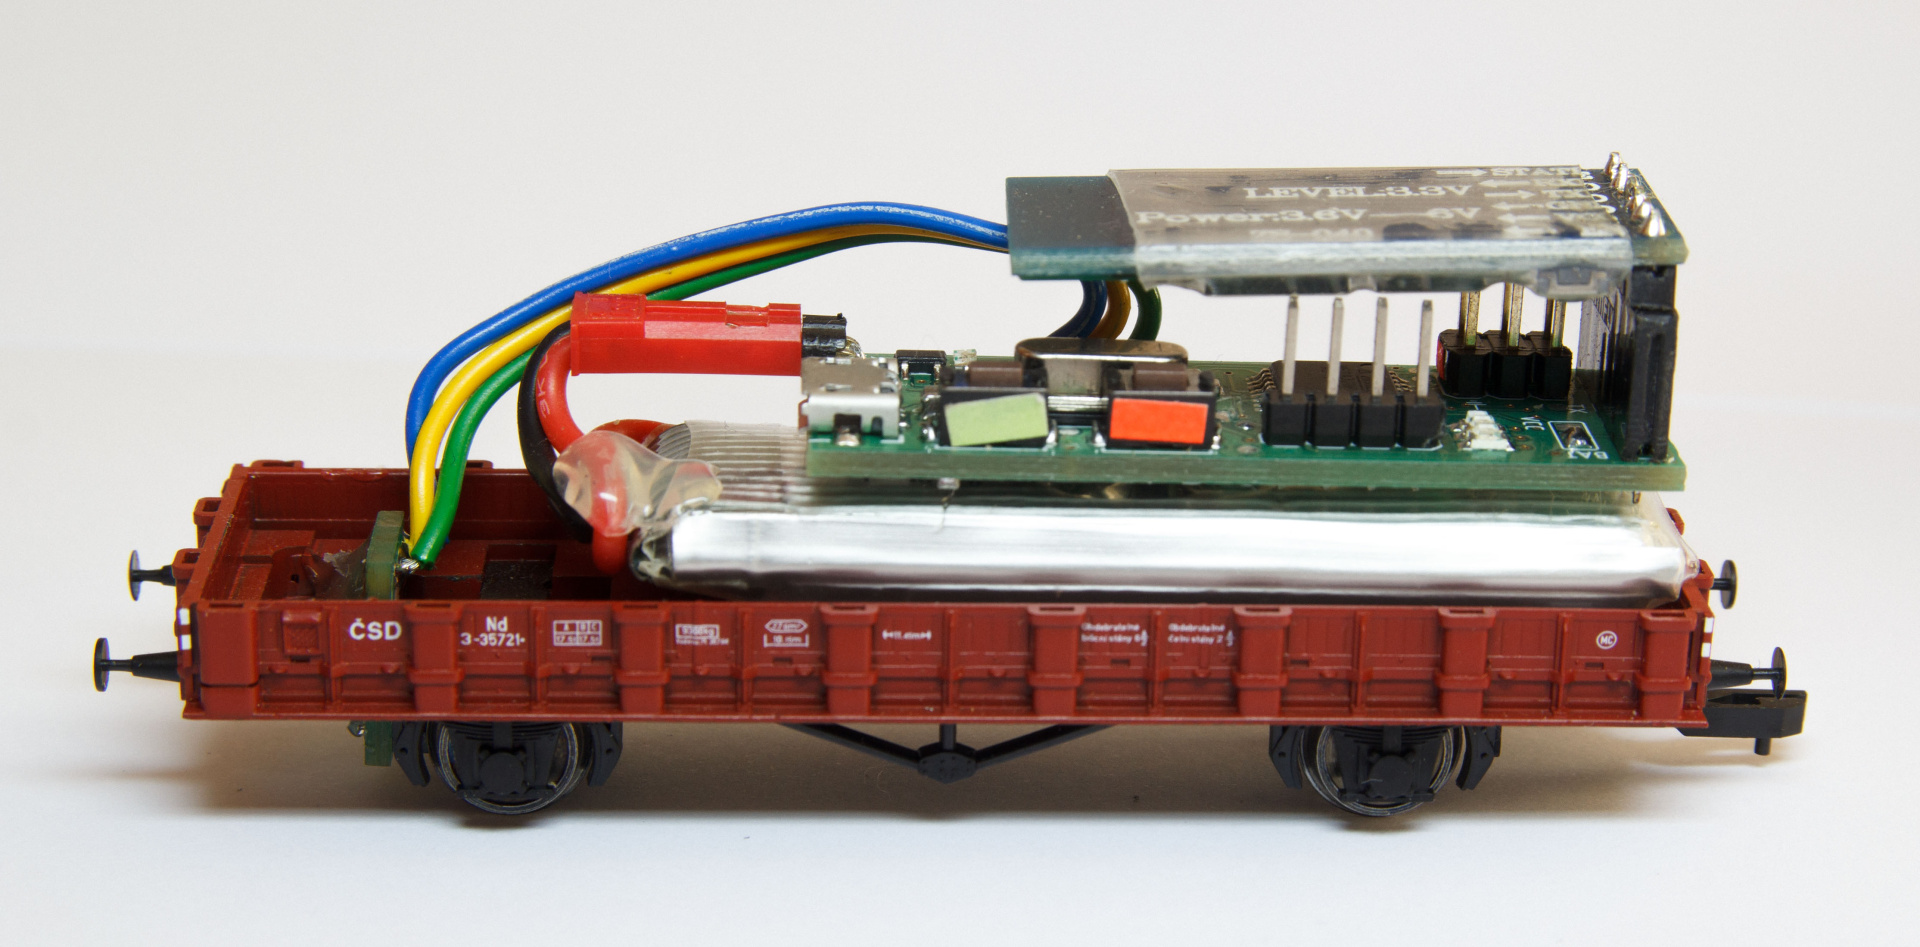
\includegraphics[width=\textwidth]{data/wsm_3d.jpg}
\caption{Fotografie prototypu měřicího vozu.}
\label{fig:vuz-photo}
\end{figure}

Tabulka \ref{tab:wsm-params} shrnuje klíčové parametry měřicího vozu.

\begin{table}
	\begin{tabularx}{\textwidth}{lrl}
		\toprule
		Parametr & Hodnota & Jednotka \\
		\midrule
		Rozměry vozu\footnote & 98 $\times$ 25 & mm \\
		Spotřeba vozu při nespárovaném BT & 55 & mA \\
		Spotřeba vozu při spárovaném BT & 33 & mA \\
		Kapacita baterie & 500 & mAh \\
		Výdrž baterie & 14 & h \\
		Pracovní napětí baterie & 3.5 -- 4.2 & V \\
		Využitá kapacita baterie & > 90 & \% \\
		Minimální měřitelná rychlost & 4 & modelový km/h\\
		Maximální měřitelná rychlost\footnote & 300 & modelový
		km/h\\
		Odhadovaná cena elektroniky & 500 & Kč\\
		\bottomrule
	\end{tabularx}
	\caption{Přehled základních parametrů měřicího vozu.}
	\label{tab:wsm-params}
\footnotetext[1]{Rozměr přes nárazníky.}
\footnotetext[2]{Účelové omezení ve firmwaru,
senzor zvládá měřit alespoň do 1000 modelových km/h}
\end{table}

Finální podobu vozu ovlivňovaly nejvíce ze všeho požadavky na malé rozměry všech
komponent měřicího vozu, dalším důležitým faktorem pak bylo napájení -- tedy
sehnat takovou baterii, která se do vozu vhodně vejde a~poskytne kapacitu
alespoň na několik hodin kalibrace.

Po vyrobení vozu byla provedena \uv{kalibrace} samotného vozu -- tedy určení
konstant uvedených ve vztahu \ref{prepocet}. Pro dosažení maximální přesnosti
se totiž nelze spoléhat zejména na měření průměru kola pouhým posuvným
měřidlem, rozdíly v~průměru kola v~řádu setin milimetru totiž způsobují rozdíly
v~modelové rychlosti v~řádu desetin modelových km/h. Autor tedy přistoupil ke
změření počtu pulzů na rovné koleji o~délce 1 m\footnote{Délka byla měřena
konvenčním svinovacím metrem.}. Postupně byly naměřeny hodnoty $317$, $317$,
$316$, $316$ a~$316$. První tři hodnoty byly měřeny na jednom úseku trati
v~různých směrech pohybu, zbylé 2 hodnoty byly pro eliminaci chyby měřeny na
jiném úseku trati, opět každá hodnota v~jiném směru pohybu vozu v~úseku a~na
rovné koleji bez jakýchkoliv nerovností.

Po zprůměrování pěti měření byl tedy průměr kola dle vztahu \ref{real-dist}
stanoven na $8.05\ mm$, kterážto konstanta je použita v~budoucích programech.

\section{Naměřená data}
\label{sec:wsm-data}

Měření rychlosti se ukázalo býti funkčním, vůz pravidelně posílal naměřená
data, rychlost se pohybovala v~odhadovaných intervalech. V~naměřených datech
byla ale vidět poměrně silná oscilace rychlosti, jejíž perioda byla řádově
\textit{vyšší desetiny sekundy}. Tato oscilace vykazovala amplitudu až
modelových 5 km/h, což je pro účely kalibrace zcela nevyhovující.

Autor tedy přistoupil ke zkoumání příčin této oscilace a~snaze o~jejich
odstranění. Autor upravil firmware v~procesoru tak, aby zasílal do počítače
každou naměřenou hodnotu a~v~počítači tak bylo možné vyhodnocovat surová data.

Při jemnějším pohledu na pohybující se vůz si šlo všimnout, že vůz ve spřáhlu
s~lokomotivou poměrně intenzivně pruží. To je dáno jak mechanickou konstrukcí
spřáhla, tak tím, že vůz i~lokomotiva obsahují kinematiku\footnote{Kinematika
je mechanismus uchycení spřáhla v~lokomotivě, ve kterém je spřáhlo k~rámu
lokomotivy připevněno přes pružiny, které zaručují natočení spřáhla při
průjezdu obloukem.}.
Autor tedy přistoupil k~nahrazení spřáhla za spřáhlo pevné. Tento krok pomohl
ke snížení amplitudy oscilace, avšak oscilace rychlosti byla nadále přítomná.

Ukázalo se tedy, že pro efektivní proces kalibrace bude nutné na kalibrované
lokomotivě vždy vyměnit spřáhlo. Toto zjištění je nepříjemné, neboť
jakákoliv nadbytečná manipulace s~kalibrovaným modelem zvyšuje šanci jeho
poškození, pragmaticky vzato však autor usuzuje, že se jedná o~přijatelné
riziko. Dnešní lokomotivy jsou na výměnu spřáhla dobře uzpůsobené, spřáhla
typicky bývají v~šachtách a~tak výměna spřáhla nepřináší až tak velká rizika.

Další zvažovanou možností bylo vůz tlačit přímo \uv{nárazník na nárazník},
ukázalo se však, že pro pevné spojení s~lokomotivou by bylo třeba vůz zatížit
řádově o~vyšší desítky gramů, což je zejména při omezených prostorech ve vozu
nereálné. Další možností je přidat soupravu se zátěží ještě před vůz a~tlačit
tak celý vlak, tuto možnost však autor vyhodnotil jako nepraktickou (bylo by
třeba mít k~dispozici další vozy, kalibrační vůz se tedy stává nekompaktní).

Naměřená data však stále vykazovala oscilaci v~řádu 5 \%, konkrétně perioda
vykazovala chybu například $2000 \pm 100$ (pro modelových 20 km/h) ticků
časovače 1. Chyba se navíc měnila s~naměřenou rychlostí a~to tak, že při
vyšších intervalech (menší rychlost) byla chyba větší než při kratších
intervalech (větší rychlost).

\begin{figure}[h]
\input{graph/speed_analog.tex}
\caption{Průběh naměřené periody a~modelové rychlosti v~čase v~analogovém
režimu.}
\label{fig:speed-analog}
\end{figure}

Graf \ref{fig:speed-analog} zachycuje průběh periody a~modelové rychlosti
v~čase. Každý celek bodů na zhruba stejné souřadnici $y$ zachycuje rychlost
vozidla při jednom napětí na jeho motoru. Rychlost je měřena na vozidlu
s~motorem připojeným přímo ke koleji (tzv. varianta \textit{analog}, bez
dekodéru), aby se eliminoval případný vliv dekodéru. Čas na ose $x$ je čas
příjmu signálu do počítače, vůči reálnému času zachycení signálu procesorem se
tento čas může mírně lišit, avšak rozdíl by měl být skutečně nepatrný.

Krom pravidelné oscilace rychlosti je na grafu místy patrný globální
\uv{obloukový} trend. Tento jev si autor vysvětluje tím, že v~průběhu měření
rychlosti vozidlo zrovna najíždělo do oblouku, takže se jeho rychlost díky
odstředivé síle zmenšila. Komentovaný jev je pro proces kalibrace parazitický,
autor se jeho vlivu obával už při prvních teoretických návrzích vozu. Později
se však ukázalo, že při kalibrování na oválu o~dostatečně velkých poloměrech
oblouků je změna rychlosti vlivem průjezdu obloukem minimální, resp. BEMF ji
okamžitě vykompenzuje. Pokud by uživatel přeci jenom chtěl kalibrovat na
obloucích o~malých poloměrech, nabízí se možnost výběru používaných a
nepoužívaných měřicích úseků na kalibračním okruhu. Stručně řečeno se bude
měřit rychlost jen ve vybraných úsecích (typicky rovných úsecích), údaj
o~poloze vozidla bude založen na vyčítání ujeté vzdálenosti vozidla, viz sekci
\ref{sec:wsm-mer-princip}.

Všimněte si v~grafu \ref{fig:speed-analog} také průběhu naměřené rychlosti.
Díky způsobu, jakým je naměřená perioda přepočítávána na modelovou rychlost
(\ref{prepocet}) dochází k~dobré eliminaci velkých chyb při malých rychlostech,
avšak chyby v~periodě u~větších rychlostí -- přestože jsou v~absolutních
hodnotách o~mnoho menší -- způsobují mnohem větší oscilace modelové rychlosti.

Pro oscilaci rychlosti bylo vytvořeno několik hypotéz.

\begin{enumerate}
\item Oscilace je způsobena nepřesností měření.

Oscilace naměřených intervalů je v~řádu stovek ticků časovače procesoru, je tedy
zřejmé, že se nemůže jednat o~chybu měření v~procesoru. Dalším zdrojem chyb
může být mechanická nepřesnost v~poloze děr v~perforovaném kole, či chyba
v~umístění kola (natočené kolo).

Pokud je tato hypotéza pravdivá, chyba v~datech by se u~měřicího vozu měla
projevit, ať už je zdrojem pohybu vozu cokoliv. Autor tedy přistoupil k~tomu,
že do vozu prostě \uv{šťouchnul} a~sledoval jeho rychlost během zpomalování.
Tuto rychlost zobrazuje graf \ref{fig:speed-zduch}.

\begin{figure}[h]
\input{graph/speed_zduch.tex}
\caption{Průběh naměřené periody zpomaleného pohybu.}
\label{fig:speed-zduch}
\end{figure}

Všimněte si, že rozsah na ose $y$ je asi $4 \times$ menší než rozsah v~grafu
\ref{fig:speed-analog}, přesto není oscilace na tomto grafu patrná.

Osilace tedy není způsobena chybou v~konstrukci měřicího vozu.

\item Oscilace je způsobena BEMF regulátorem v~dekodéru.

Jak bylo zmíněno v~kapitole \ref{sec:det-static}, každý dekodér v~sobě má PID
regulátor, který zajišťuje udržování rychlosti hnacího vozidla při rozdílném
počtu zavěšených vozů, resp. při rozdílné zátěži. Jako každý PID regulátor,
i tento regulátor nemusí být dobře nastaven, výrobce dekodéru ostatně často
vůbec netuší, do jakého modelu bude jeho dekodér osazen.

Tuto hypotézu však vyvrací fakt, že oscilace se projevuje i když měříme rychlost
vozidla bez dekodéru -- v~tzv. režimu analog, kdy připojujeme napětí v~kolejích
přímo na motor.

\item Oscilace je způsobena charakteristikou motoru a~mechanickými vlastnostmi
modelu.

\begin{figure}[h]
\input{graph/speed_detail.tex}
\caption{Detailnější pohled na oscilace rychlosti.}
\label{fig:speed-presny}
\end{figure}

Zde se pouštíme už na poměrně tenký led. Z~grafu \ref{fig:speed-presny} je
patrné, že měření frekvence oscilace je za hranou možností měřicího
vozu. Počet děr v~perforovaném kolu je na přesné měření frekvence totiž příliš
malý.

Poslední hypotézou tedy zůstává to, že oscilace, která je patrná v~grafu,
je přímým důsledkem postupné aktivace pólů motoru, střídy signálu do motoru,
případně důsledkem nedokonalých převodů lokomotivy a~šíření vibrací přes
koleje až do vozu.

Fakt, že amplituda oscilace je při nižších rychlostech vyšší lze vysvětlit tím,
že vozidlo má při nižších rychlostech menší setrvačnost a~tudíž se pulzní
charakter regulace a~nepřesnosti v~převodech více projevuje.

Jako drobnou poznámku autor uvádí, že z~jím naměřených dat nejspíš (!) plyne,
že perioda oscilace se liší u~různých vozidel. Měření na různých vozidlech
proběhlo, autor ale znovu podotýká, že měření frekvence oscilace je za hranou
možností měřicího vozu.

\end{enumerate}

\subsection{Kompenzace chyb}
\label{subsec:wsm-kompenzace}

Z~naměřených dat vyplývá, že v~signálu se vyskytuje určitá periodická chyba,
kterou by bylo vhodné kompenzovat. Za tímto účelem vznikl návrh průměrovací
metody \textit{kluzné okno}. Tato metoda je implementována v~produkční verzi
kalibračního vozu, princip její činnosti je následující:

\begin{compactenum}
\item Měř počty ticků a~jejich periodu ve $100ms$ oknech.
\item Každých $100\ ms$ přepni na nové okno.
\item Data do počítače průměruj z~posledních $10$ oken, tedy celkem z~$1\ s$.
\end{compactenum}

Tato metoda je poměrně známá, zajímavou věcí na implementaci v~měřicím vozu
jsou výše uvedené konstanty. $100\ ms$ proto, aby data v~počítači byla vidět
v~rozumně \textit{reálném čase} a~naopak příliš nezahlcovala komunikační kanál,
$1\ s$ proto, že se jedná o~latenci, kterou je uživatel ještě schopen tolerovat,
navíc za tento čas obvykle nastane alespoň jedna perioda signálu (viz naměřená
data v~grafech výše).

O~přesné přepínání oken se v~procesoru stará časovač 0.

Průběh naměřené periody a~vypočítané rychlosti za použití průměrovací metody
zachycuje graf \ref{fig:prumer}. Srovnejte s~grafem \ref{fig:speed-analog}!

\begin{figure}[h]
\input{graph/speed_prumer.tex}
\caption{Naměřená data za použití průměrovací metody.}
\label{fig:prumer}
\end{figure}
